% =============================================================================
% Lecture 5: Financial Literacy
% =============================================================================
\documentclass[9pt,english,aspectratio=169]{beamer}
% =============================================================================
% Pathways: Economics & Finance Workshop — Beamer Preamble
% =============================================================================
% Usage: Each lecture .tex file should start with:
%   \documentclass[10pt,english,aspectratio=169]{beamer}
%   % =============================================================================
% Pathways: Economics & Finance Workshop — Beamer Preamble
% =============================================================================
% Usage: Each lecture .tex file should start with:
%   \documentclass[10pt,english,aspectratio=169]{beamer}
%   % =============================================================================
% Pathways: Economics & Finance Workshop — Beamer Preamble
% =============================================================================
% Usage: Each lecture .tex file should start with:
%   \documentclass[10pt,english,aspectratio=169]{beamer}
%   \input{../../codes/Preambles/header_slides}
% Compile: cd output/Slides && TEXINPUTS=../../codes/Preambles:$TEXINPUTS xelatex file.tex
% =============================================================================

% ---------- Packages ----------
% Fonts
\usepackage{lmodern}
\usepackage[utf8]{inputenc}
\usepackage[normalem]{ulem}

% Math
\usepackage{amsmath,amssymb,amsthm}

% Figures and tables
\usepackage{graphicx}
\usepackage{array,tabularx,booktabs,threeparttable}

% TikZ and pgfplots
\usepackage{pgfplots}
\pgfplotsset{compat=1.18}
\usepackage{tikz}
\usetikzlibrary{positioning,arrows.meta,calc}

% Colored boxes
\usepackage[most]{tcolorbox}

% Miscellaneous
\usepackage{transparent}
\usepackage{setspace}
\usepackage[nodayofweek]{datetime}
\usepackage{hyperref}

% ---------- Theme ----------
\usetheme{CambridgeUS}
\usecolortheme{dolphin}
\usepackage{appendixnumberbeamer}

% ---------- Itemize ----------
\setbeamercovered{invisible}
\setbeamertemplate{itemize items}[default]
\setbeamertemplate{enumerate items}[default]

\setbeamertemplate{itemize item}[triangle]
\setbeamertemplate{itemize subitem}[triangle]
\setbeamertemplate{itemize subsubitem}{-}

% ---------- Headline / Footline ----------
\setbeamertemplate{headline}{}

\setbeamertemplate{footline}{
  \leavevmode
  \hbox{
    \begin{beamercolorbox}[wd=\paperwidth,ht=2.5ex,dp=1.25ex,leftskip=1em,rightskip=1em]{footline}
      \hfill \insertframenumber
    \end{beamercolorbox}
  }
}

\setbeamertemplate{navigation symbols}{}

% ---------- Frame title (centered) ----------
\makeatletter
\setbeamertemplate{frametitle}{
  \nointerlineskip
  \begin{beamercolorbox}[wd=\paperwidth,sep=0.35cm,center]{frametitle}
    {\usebeamerfont{frametitle}\insertframetitle\par}
    \ifx\insertframesubtitle\@empty\else
      \vspace{0.15cm}
      {\usebeamerfont{framesubtitle}\usebeamercolor[fg]{framesubtitle}\insertframesubtitle\par}
    \fi
  \end{beamercolorbox}
}
\makeatother

% ---------- Margins ----------
\setbeamersize{
  text margin left=2em,
  text margin right=2em
}

% ---------- Section outline frames ----------
\AtBeginSection[]{
  \begin{frame}{Outline}
    \tableofcontents[currentsection,
                     currentsubsection,
                     hideothersubsections]
  \end{frame}
}

% =============================================================================
% Colors — Okabe-Ito colorblind-friendly palette
% =============================================================================

\definecolor{black}{HTML}{000000}
\definecolor{orange}{HTML}{E69F00}
\definecolor{skyblue}{HTML}{56B4E9}
\definecolor{green}{HTML}{009E73}
\definecolor{yellow}{HTML}{F0E442}
\definecolor{blue}{HTML}{0072B2}
\definecolor{vermillion}{HTML}{D55E00}
\definecolor{purple}{HTML}{CC79A7}

% Semantic aliases (mapped to Okabe-Ito)
\definecolor{softbg}{HTML}{F5F5F5}
\definecolor{lightgray}{gray}{0.65}

% =============================================================================
% Box Environments
% =============================================================================

% --- Key points (orange background) ---
\newtcolorbox{keybox}{
  colback=orange!12,
  colframe=orange,
  fonttitle=\bfseries,
  boxrule=0.5pt,
  arc=2pt,
  left=6pt,
  right=6pt,
  top=4pt,
  bottom=4pt
}

% --- Highlights (orange left accent) ---
\newtcolorbox{highlightbox}{
  colback=white,
  colframe=orange,
  fonttitle=\bfseries,
  boxrule=0pt,
  leftrule=3pt,
  arc=0pt,
  left=6pt,
  right=6pt,
  top=4pt,
  bottom=4pt
}

% --- Definitions (blue border, titled) ---
\newtcolorbox{definitionbox}[1][]{
  colback=blue!5,
  colframe=blue,
  fonttitle=\bfseries,
  title={#1},
  boxrule=0.5pt,
  arc=2pt,
  left=6pt,
  right=6pt,
  top=4pt,
  bottom=4pt
}

% --- Methods (sky blue background) ---
\newtcolorbox{methodbox}{
  colback=skyblue!8,
  colframe=skyblue!70,
  fonttitle=\bfseries,
  boxrule=0.5pt,
  arc=2pt,
  left=6pt,
  right=6pt,
  top=4pt,
  bottom=4pt
}

% --- Results (green border) ---
\newtcolorbox{resultbox}{
  colback=green!5,
  colframe=green,
  fonttitle=\bfseries,
  boxrule=0.5pt,
  arc=2pt,
  left=6pt,
  right=6pt,
  top=4pt,
  bottom=4pt
}

% --- Quotes (purple left rule) ---
\newtcolorbox{quotebox}{
  colback=softbg,
  colframe=purple,
  fonttitle=\itshape,
  boxrule=0pt,
  leftrule=2pt,
  arc=0pt,
  left=6pt,
  right=6pt,
  top=4pt,
  bottom=4pt
}

% =============================================================================
% Math Commands
% =============================================================================

\newcommand{\E}{\mathrm{E}}
\newcommand{\Var}{\mathrm{Var}}
\newcommand{\Cov}{\mathrm{Cov}}
\newcommand{\R}{\mathbb{R}}
\newcommand{\suminfty}[1]{\sum_{#1=0}^\infty}
\newcommand{\Lcal}{\mathcal{L}}
\newcommand{\prtl}[2]{\frac{\partial #1}{\partial #2}}
\renewcommand{\div}[2]{\frac{d #1}{d #2}}
\newcommand{\suchthat}{\text{ s.t. }}
\newcommand{\wrt}{\text{ w.r.t. }}
\newcommand{\red}[1]{\textcolor{vermillion}{#1}}
\newcommand{\blue}[1]{\textcolor{blue}{#1}}

% =============================================================================
% Economics Shortcuts
% =============================================================================

\newcommand{\OC}{\text{Opportunity Cost}}
\newcommand{\DWL}{\text{DWL}}
\newcommand{\pmark}{\textcolor{resultgreen}{\checkmark}}
\newcommand{\xmark}{\textcolor{darkred}{\texttimes}}

% Compile: cd output/Slides && TEXINPUTS=../../codes/Preambles:$TEXINPUTS xelatex file.tex
% =============================================================================

% ---------- Packages ----------
% Fonts
\usepackage{lmodern}
\usepackage[utf8]{inputenc}
\usepackage[normalem]{ulem}

% Math
\usepackage{amsmath,amssymb,amsthm}

% Figures and tables
\usepackage{graphicx}
\usepackage{array,tabularx,booktabs,threeparttable}

% TikZ and pgfplots
\usepackage{pgfplots}
\pgfplotsset{compat=1.18}
\usepackage{tikz}
\usetikzlibrary{positioning,arrows.meta,calc}

% Colored boxes
\usepackage[most]{tcolorbox}

% Miscellaneous
\usepackage{transparent}
\usepackage{setspace}
\usepackage[nodayofweek]{datetime}
\usepackage{hyperref}

% ---------- Theme ----------
\usetheme{CambridgeUS}
\usecolortheme{dolphin}
\usepackage{appendixnumberbeamer}

% ---------- Itemize ----------
\setbeamercovered{invisible}
\setbeamertemplate{itemize items}[default]
\setbeamertemplate{enumerate items}[default]

\setbeamertemplate{itemize item}[triangle]
\setbeamertemplate{itemize subitem}[triangle]
\setbeamertemplate{itemize subsubitem}{-}

% ---------- Headline / Footline ----------
\setbeamertemplate{headline}{}

\setbeamertemplate{footline}{
  \leavevmode
  \hbox{
    \begin{beamercolorbox}[wd=\paperwidth,ht=2.5ex,dp=1.25ex,leftskip=1em,rightskip=1em]{footline}
      \hfill \insertframenumber
    \end{beamercolorbox}
  }
}

\setbeamertemplate{navigation symbols}{}

% ---------- Frame title (centered) ----------
\makeatletter
\setbeamertemplate{frametitle}{
  \nointerlineskip
  \begin{beamercolorbox}[wd=\paperwidth,sep=0.35cm,center]{frametitle}
    {\usebeamerfont{frametitle}\insertframetitle\par}
    \ifx\insertframesubtitle\@empty\else
      \vspace{0.15cm}
      {\usebeamerfont{framesubtitle}\usebeamercolor[fg]{framesubtitle}\insertframesubtitle\par}
    \fi
  \end{beamercolorbox}
}
\makeatother

% ---------- Margins ----------
\setbeamersize{
  text margin left=2em,
  text margin right=2em
}

% ---------- Section outline frames ----------
\AtBeginSection[]{
  \begin{frame}{Outline}
    \tableofcontents[currentsection,
                     currentsubsection,
                     hideothersubsections]
  \end{frame}
}

% =============================================================================
% Colors — Okabe-Ito colorblind-friendly palette
% =============================================================================

\definecolor{black}{HTML}{000000}
\definecolor{orange}{HTML}{E69F00}
\definecolor{skyblue}{HTML}{56B4E9}
\definecolor{green}{HTML}{009E73}
\definecolor{yellow}{HTML}{F0E442}
\definecolor{blue}{HTML}{0072B2}
\definecolor{vermillion}{HTML}{D55E00}
\definecolor{purple}{HTML}{CC79A7}

% Semantic aliases (mapped to Okabe-Ito)
\definecolor{softbg}{HTML}{F5F5F5}
\definecolor{lightgray}{gray}{0.65}

% =============================================================================
% Box Environments
% =============================================================================

% --- Key points (orange background) ---
\newtcolorbox{keybox}{
  colback=orange!12,
  colframe=orange,
  fonttitle=\bfseries,
  boxrule=0.5pt,
  arc=2pt,
  left=6pt,
  right=6pt,
  top=4pt,
  bottom=4pt
}

% --- Highlights (orange left accent) ---
\newtcolorbox{highlightbox}{
  colback=white,
  colframe=orange,
  fonttitle=\bfseries,
  boxrule=0pt,
  leftrule=3pt,
  arc=0pt,
  left=6pt,
  right=6pt,
  top=4pt,
  bottom=4pt
}

% --- Definitions (blue border, titled) ---
\newtcolorbox{definitionbox}[1][]{
  colback=blue!5,
  colframe=blue,
  fonttitle=\bfseries,
  title={#1},
  boxrule=0.5pt,
  arc=2pt,
  left=6pt,
  right=6pt,
  top=4pt,
  bottom=4pt
}

% --- Methods (sky blue background) ---
\newtcolorbox{methodbox}{
  colback=skyblue!8,
  colframe=skyblue!70,
  fonttitle=\bfseries,
  boxrule=0.5pt,
  arc=2pt,
  left=6pt,
  right=6pt,
  top=4pt,
  bottom=4pt
}

% --- Results (green border) ---
\newtcolorbox{resultbox}{
  colback=green!5,
  colframe=green,
  fonttitle=\bfseries,
  boxrule=0.5pt,
  arc=2pt,
  left=6pt,
  right=6pt,
  top=4pt,
  bottom=4pt
}

% --- Quotes (purple left rule) ---
\newtcolorbox{quotebox}{
  colback=softbg,
  colframe=purple,
  fonttitle=\itshape,
  boxrule=0pt,
  leftrule=2pt,
  arc=0pt,
  left=6pt,
  right=6pt,
  top=4pt,
  bottom=4pt
}

% =============================================================================
% Math Commands
% =============================================================================

\newcommand{\E}{\mathrm{E}}
\newcommand{\Var}{\mathrm{Var}}
\newcommand{\Cov}{\mathrm{Cov}}
\newcommand{\R}{\mathbb{R}}
\newcommand{\suminfty}[1]{\sum_{#1=0}^\infty}
\newcommand{\Lcal}{\mathcal{L}}
\newcommand{\prtl}[2]{\frac{\partial #1}{\partial #2}}
\renewcommand{\div}[2]{\frac{d #1}{d #2}}
\newcommand{\suchthat}{\text{ s.t. }}
\newcommand{\wrt}{\text{ w.r.t. }}
\newcommand{\red}[1]{\textcolor{vermillion}{#1}}
\newcommand{\blue}[1]{\textcolor{blue}{#1}}

% =============================================================================
% Economics Shortcuts
% =============================================================================

\newcommand{\OC}{\text{Opportunity Cost}}
\newcommand{\DWL}{\text{DWL}}
\newcommand{\pmark}{\textcolor{resultgreen}{\checkmark}}
\newcommand{\xmark}{\textcolor{darkred}{\texttimes}}

% Compile: cd output/Slides && TEXINPUTS=../../codes/Preambles:$TEXINPUTS xelatex file.tex
% =============================================================================

% ---------- Packages ----------
% Fonts
\usepackage{lmodern}
\usepackage[utf8]{inputenc}
\usepackage[normalem]{ulem}

% Math
\usepackage{amsmath,amssymb,amsthm}

% Figures and tables
\usepackage{graphicx}
\usepackage{array,tabularx,booktabs,threeparttable}

% TikZ and pgfplots
\usepackage{pgfplots}
\pgfplotsset{compat=1.18}
\usepackage{tikz}
\usetikzlibrary{positioning,arrows.meta,calc}

% Colored boxes
\usepackage[most]{tcolorbox}

% Miscellaneous
\usepackage{transparent}
\usepackage{setspace}
\usepackage[nodayofweek]{datetime}
\usepackage{hyperref}

% ---------- Theme ----------
\usetheme{CambridgeUS}
\usecolortheme{dolphin}
\usepackage{appendixnumberbeamer}

% ---------- Itemize ----------
\setbeamercovered{invisible}
\setbeamertemplate{itemize items}[default]
\setbeamertemplate{enumerate items}[default]

\setbeamertemplate{itemize item}[triangle]
\setbeamertemplate{itemize subitem}[triangle]
\setbeamertemplate{itemize subsubitem}{-}

% ---------- Headline / Footline ----------
\setbeamertemplate{headline}{}

\setbeamertemplate{footline}{
  \leavevmode
  \hbox{
    \begin{beamercolorbox}[wd=\paperwidth,ht=2.5ex,dp=1.25ex,leftskip=1em,rightskip=1em]{footline}
      \hfill \insertframenumber
    \end{beamercolorbox}
  }
}

\setbeamertemplate{navigation symbols}{}

% ---------- Frame title (centered) ----------
\makeatletter
\setbeamertemplate{frametitle}{
  \nointerlineskip
  \begin{beamercolorbox}[wd=\paperwidth,sep=0.35cm,center]{frametitle}
    {\usebeamerfont{frametitle}\insertframetitle\par}
    \ifx\insertframesubtitle\@empty\else
      \vspace{0.15cm}
      {\usebeamerfont{framesubtitle}\usebeamercolor[fg]{framesubtitle}\insertframesubtitle\par}
    \fi
  \end{beamercolorbox}
}
\makeatother

% ---------- Margins ----------
\setbeamersize{
  text margin left=2em,
  text margin right=2em
}

% ---------- Section outline frames ----------
\AtBeginSection[]{
  \begin{frame}{Outline}
    \tableofcontents[currentsection,
                     currentsubsection,
                     hideothersubsections]
  \end{frame}
}

% =============================================================================
% Colors — Okabe-Ito colorblind-friendly palette
% =============================================================================

\definecolor{black}{HTML}{000000}
\definecolor{orange}{HTML}{E69F00}
\definecolor{skyblue}{HTML}{56B4E9}
\definecolor{green}{HTML}{009E73}
\definecolor{yellow}{HTML}{F0E442}
\definecolor{blue}{HTML}{0072B2}
\definecolor{vermillion}{HTML}{D55E00}
\definecolor{purple}{HTML}{CC79A7}

% Semantic aliases (mapped to Okabe-Ito)
\definecolor{softbg}{HTML}{F5F5F5}
\definecolor{lightgray}{gray}{0.65}

% =============================================================================
% Box Environments
% =============================================================================

% --- Key points (orange background) ---
\newtcolorbox{keybox}{
  colback=orange!12,
  colframe=orange,
  fonttitle=\bfseries,
  boxrule=0.5pt,
  arc=2pt,
  left=6pt,
  right=6pt,
  top=4pt,
  bottom=4pt
}

% --- Highlights (orange left accent) ---
\newtcolorbox{highlightbox}{
  colback=white,
  colframe=orange,
  fonttitle=\bfseries,
  boxrule=0pt,
  leftrule=3pt,
  arc=0pt,
  left=6pt,
  right=6pt,
  top=4pt,
  bottom=4pt
}

% --- Definitions (blue border, titled) ---
\newtcolorbox{definitionbox}[1][]{
  colback=blue!5,
  colframe=blue,
  fonttitle=\bfseries,
  title={#1},
  boxrule=0.5pt,
  arc=2pt,
  left=6pt,
  right=6pt,
  top=4pt,
  bottom=4pt
}

% --- Methods (sky blue background) ---
\newtcolorbox{methodbox}{
  colback=skyblue!8,
  colframe=skyblue!70,
  fonttitle=\bfseries,
  boxrule=0.5pt,
  arc=2pt,
  left=6pt,
  right=6pt,
  top=4pt,
  bottom=4pt
}

% --- Results (green border) ---
\newtcolorbox{resultbox}{
  colback=green!5,
  colframe=green,
  fonttitle=\bfseries,
  boxrule=0.5pt,
  arc=2pt,
  left=6pt,
  right=6pt,
  top=4pt,
  bottom=4pt
}

% --- Quotes (purple left rule) ---
\newtcolorbox{quotebox}{
  colback=softbg,
  colframe=purple,
  fonttitle=\itshape,
  boxrule=0pt,
  leftrule=2pt,
  arc=0pt,
  left=6pt,
  right=6pt,
  top=4pt,
  bottom=4pt
}

% =============================================================================
% Math Commands
% =============================================================================

\newcommand{\E}{\mathrm{E}}
\newcommand{\Var}{\mathrm{Var}}
\newcommand{\Cov}{\mathrm{Cov}}
\newcommand{\R}{\mathbb{R}}
\newcommand{\suminfty}[1]{\sum_{#1=0}^\infty}
\newcommand{\Lcal}{\mathcal{L}}
\newcommand{\prtl}[2]{\frac{\partial #1}{\partial #2}}
\renewcommand{\div}[2]{\frac{d #1}{d #2}}
\newcommand{\suchthat}{\text{ s.t. }}
\newcommand{\wrt}{\text{ w.r.t. }}
\newcommand{\red}[1]{\textcolor{vermillion}{#1}}
\newcommand{\blue}[1]{\textcolor{blue}{#1}}

% =============================================================================
% Economics Shortcuts
% =============================================================================

\newcommand{\OC}{\text{Opportunity Cost}}
\newcommand{\DWL}{\text{DWL}}
\newcommand{\pmark}{\textcolor{resultgreen}{\checkmark}}
\newcommand{\xmark}{\textcolor{darkred}{\texttimes}}


% ---------- Title ----------
\title{\textbf{Financial Literacy}}
\subtitle{Pathways to Arts \& Humanities Summer Scholars Program}
\author{Instructor: Tudor Schlanger}
\date{Summer 2026}

\begin{document}

% =============================================================================
% Title
% =============================================================================
\begin{frame}
  \titlepage
\end{frame}

% =============================================================================
% Opening Quiz
% =============================================================================

\begin{frame}{What Is Financial Literacy?}

  \vspace{0.6em}
  \begin{columns}[T]
    \begin{column}{0.58\textwidth}
     \begin{definitionbox}[Financial Literacy]
    The ability to understand and use everyday money skills, e.g. \textbf{saving},
    \textbf{borrowing}, and \textbf{investing}. 
    \end{definitionbox}
        \pause
        \vspace{1em}
      \textbf{Why does it matter?}
      \begin{itemize}
        \item Everyone deals with money.
        \item Making good decisions builds wealth. 
        \item Mistakes are expensive!
      \end{itemize}

    \end{column}
    \begin{column}{0.38\textwidth}
      \vspace{0.5em}
      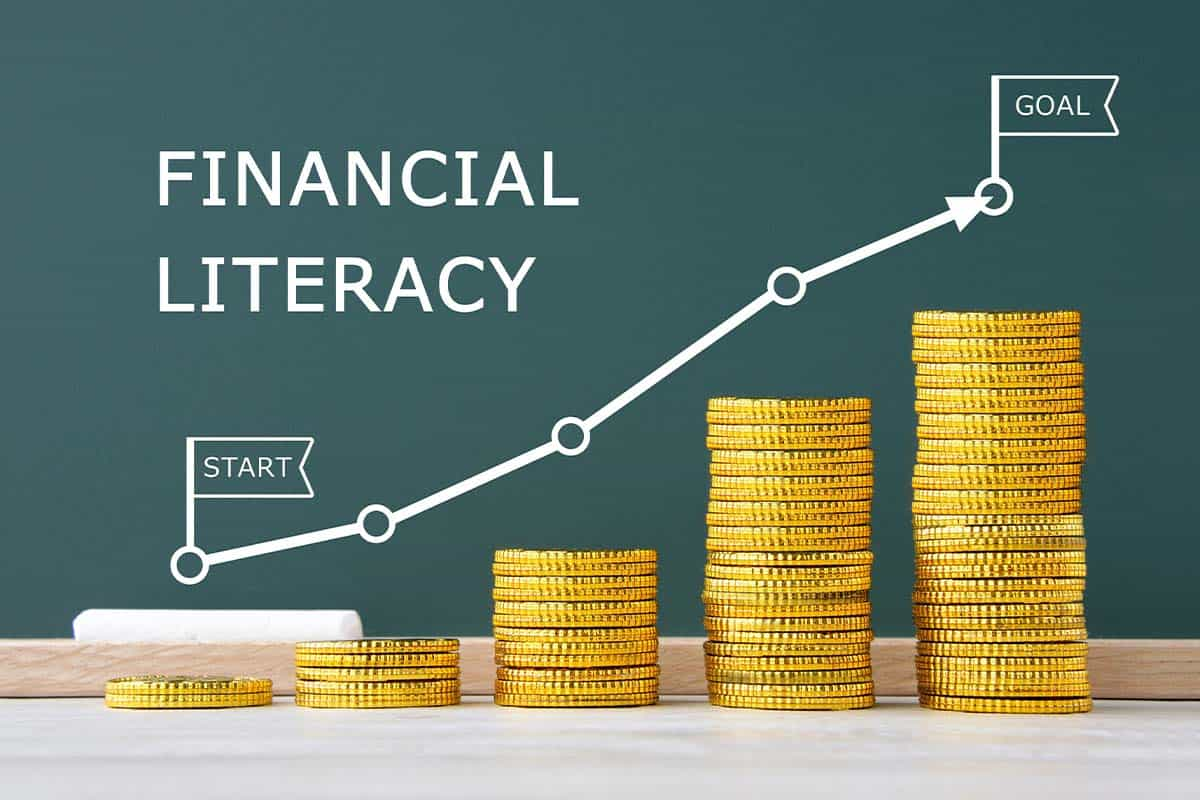
\includegraphics[width=\textwidth]{fig/fin_literacy.jpg}

      \vspace{0.3em}
    \end{column}
  \end{columns}

\end{frame}

\begin{frame}{Quiz: Question 1 of 4}

  \begin{questionbox}
    Suppose you had \$100 in a savings account and the interest rate was 2\%
    per year. After 5 years, how much do you think you would have in the
    account if you left the money to grow?
  \end{questionbox}

  \vspace{1em}
  \setbeamertemplate{enumerate item}{\Alph{enumi}.}
  \begin{enumerate}
    \item More than \$102
    \item Exactly \$102
    \item Less than \$102
    \item Do not know
  \end{enumerate}

\end{frame}

\begin{frame}{Quiz: Question 2 of 4}

  \begin{questionbox}
    Imagine that the interest rate on your savings account was 1\% per year
    and inflation was 2\% per year. After 1 year, how much would you be able
    to buy with the money in this account?
  \end{questionbox}

  \vspace{1em}
  \setbeamertemplate{enumerate item}{\Alph{enumi}.}
  \begin{enumerate}
    \item More than today
    \item Exactly the same
    \item Less than today
    \item Do not know
  \end{enumerate}

\end{frame}

\begin{frame}{Quiz: Question 3 of 4}

  \begin{questionbox}
    If interest rates rise, what should happen to bond prices?
  \end{questionbox}

  \vspace{1em}
  \setbeamertemplate{enumerate item}{\Alph{enumi}.}
  \begin{enumerate}
    \item They should rise
    \item They should fall
    \item They should stay the same
    \item There is no relationship between bond prices and interest rates
    \item Do not know
  \end{enumerate}

\end{frame}

\begin{frame}{Quiz: Question 4 of 4}

  \begin{questionbox}
    Please tell me whether this statement is true or false: ``Buying a single
    company's stock usually provides a safer return than a stock mutual fund.''
  \end{questionbox}

  \vspace{1em}
  \setbeamertemplate{enumerate item}{\Alph{enumi}.}
  \begin{enumerate}
    \item True
    \item False
    \item Do not know
  \end{enumerate}

\end{frame}

% =============================================================================
\section{Saving \& Compound Interest}
% =============================================================================

\begin{frame}{What Is Saving?}

  \begin{columns}[T]
    \begin{column}{0.5\textwidth}
      \begin{definitionbox}[Saving]
        Setting aside part of your income today so you can use it in the future.
      \end{definitionbox}

      \vspace{0.8em}
      \textbf{Why do we need to save?}
      \begin{itemize}
        \item Big future purchases (college, car, house)
        \item Retirement (you won't work forever!)
        \item Emergencies (unexpected expenses)
      \end{itemize}

    \end{column}
    \begin{column}{0.45\textwidth}
      \vspace{1em}
      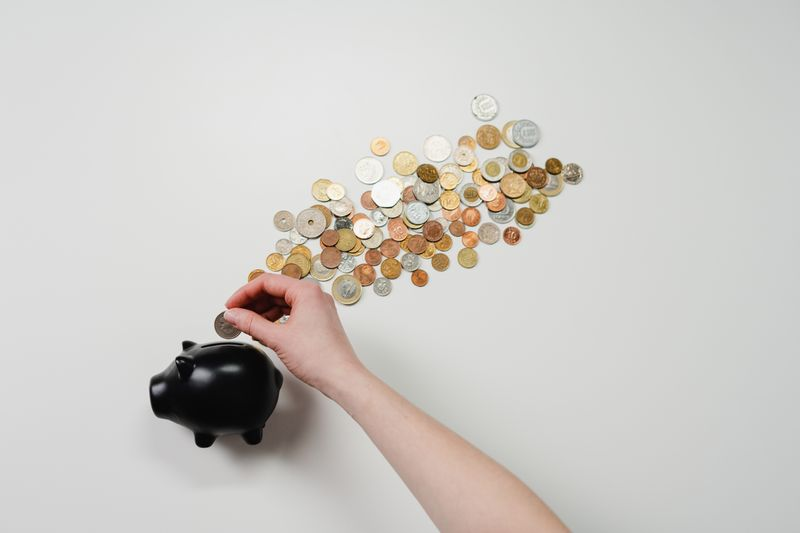
\includegraphics[width=\textwidth]{fig/piggy_bank.jpg}

      \vspace{0.3em}
      {\tiny\textcolor{lightgray}{Photo: Pexels (free license)}}
    \end{column}
  \end{columns}
  \pause
  \begin{columns}[T]
    \begin{column}{0.5\textwidth}

\begin{questionbox}
  How do we \textbf{save}?
\end{questionbox}
       \end{column}\pause  

    \begin{column}{0.45\textwidth}
\begin{answerbox}
   By putting money into \textbf{assets}.
\end{answerbox}
          \end{column}
  \end{columns}

\end{frame}

\begin{frame}{Types of Assets}

  \begin{columns}[T]
    \begin{column}{0.45\textwidth}
      \textcolor{blue}{\textbf{Financial Assets}}
      \begin{itemize}
        \item Savings accounts
        \item Bonds
        \item Stocks
      \end{itemize}
    \end{column}
    \begin{column}{0.45\textwidth}
      \textcolor{orange}{\textbf{Non-Financial Assets}}
      \begin{itemize}
        \item House
        \item Car
        \item Land
      \end{itemize}
    \end{column}
  \end{columns}
  \pause
  \vspace{1.5em}
  How to tell them apart:
  \begin{itemize}
    \item \textbf{Tangibility:} non-financial assets are physical, you can touch a house, but not a stock
    \item \textbf{Liquidity:} financial assets are easy to sell quickly (click a button); selling a house takes months
  \end{itemize}
  \vspace{1em}

  \pause 
  \begin{questionbox}
    How are these financial assets different? 
  \end{questionbox}

\end{frame}

\begin{frame}{Financial Assets}

  \begin{columns}[T]
    \begin{column}{0.45\textwidth}
      \vspace{0.5em}
      \begin{tikzpicture}
        \begin{axis}[
          width=6.5cm, height=6cm,
          xlabel={Riskiness}, ylabel={Expected Return},
          xmin=0, xmax=10, ymin=0, ymax=10,
          xtick=\empty, ytick=\empty,
          xlabel style={font=\small}, ylabel style={font=\small},
          axis lines=left,
          clip=false,
        ]
        \end{axis}
      \end{tikzpicture}
    \end{column}
    \begin{column}{0.50\textwidth}
      \begin{itemize}
        \item \textcolor{blue}{\textbf{Expected return:}} how much you \emph{typically} expect your money to grow. Put in \$100, get back \$105 in a year? That's a 5\% return.

        \vspace{0.75em}
        \item \textcolor{vermillion}{\textbf{Riskiness:}} how \emph{uncertain} that return is. A safe bet pays about what you expect; a risky one might soar\ldots or lose money.
      \end{itemize}
    \end{column}
  \end{columns}

\end{frame}

\begin{frame}{Financial Assets}

  \begin{columns}[T]
    \begin{column}{0.45\textwidth}
      \vspace{0.5em}
      \begin{tikzpicture}
        \begin{axis}[
          width=6.5cm, height=6cm,
          xlabel={Riskiness}, ylabel={Expected Return},
          xmin=0, xmax=10, ymin=0, ymax=10,
          xtick=\empty, ytick=\empty,
          xlabel style={font=\small}, ylabel style={font=\small},
          axis lines=left,
          clip=false,
        ]
          \addplot[dashed, DarkGray, thin, domain=0.5:9] {0.8*x + 0.5};
          \node[circle, fill=green, minimum size=10pt, inner sep=0pt] at (1.5, 1.5) {};
          \node[font=\scriptsize, anchor=north] at (1.5, 1.1) {Savings};
        \end{axis}
      \end{tikzpicture}
    \end{column}
    \begin{column}{0.50\textwidth}
      \begin{itemize}
        \item \textcolor{green}{\textbf{Savings account:}} You deposit money at a bank. They pay you a small interest rate. Very safe, very low return.
      \end{itemize}
    \end{column}
  \end{columns}

\end{frame}

\begin{frame}{Financial Assets}

  \begin{columns}[T]
    \begin{column}{0.45\textwidth}
      \vspace{0.5em}
      \begin{tikzpicture}
        \begin{axis}[
          width=6.5cm, height=6cm,
          xlabel={Riskiness}, ylabel={Expected Return},
          xmin=0, xmax=10, ymin=0, ymax=10,
          xtick=\empty, ytick=\empty,
          xlabel style={font=\small}, ylabel style={font=\small},
          axis lines=left,
          clip=false,
        ]
          \addplot[dashed, DarkGray, thin, domain=0.5:9] {0.8*x + 0.5};
          \node[circle, fill=green, minimum size=10pt, inner sep=0pt] at (1.5, 1.5) {};
          \node[font=\scriptsize, anchor=north] at (1.5, 1.1) {Savings};
          \node[circle, fill=blue, minimum size=10pt, inner sep=0pt] at (4, 4) {};
          \node[font=\scriptsize, anchor=north] at (4, 3.6) {Bond};
        \end{axis}
      \end{tikzpicture}
    \end{column}
    \begin{column}{0.50\textwidth}
      \begin{itemize}
        \item \textcolor{green}{\textbf{Savings account:}} You deposit money at a bank. They pay you a small interest rate. Very safe, very low return.

        \vspace{0.5em}
        \item \textcolor{blue}{\textbf{Bond:}} You lend money to the government or a company. They pay you back with interest. Safe, moderate interest rate.
      \end{itemize}
    \end{column}
  \end{columns}

\end{frame}

\begin{frame}{Financial Assets}

  \begin{columns}[T]
    \begin{column}{0.45\textwidth}
      \vspace{0.5em}
      \begin{tikzpicture}
        \begin{axis}[
          width=6.5cm, height=6cm,
          xlabel={Riskiness}, ylabel={Expected Return},
          xmin=0, xmax=10, ymin=0, ymax=10,
          xtick=\empty, ytick=\empty,
          xlabel style={font=\small}, ylabel style={font=\small},
          axis lines=left,
          clip=false,
        ]
          \addplot[dashed, DarkGray, thin, domain=0.5:9] {0.8*x + 0.5};
          \node[circle, fill=green, minimum size=10pt, inner sep=0pt] at (1.5, 1.5) {};
          \node[font=\scriptsize, anchor=north] at (1.5, 1.1) {Savings};
          \node[circle, fill=blue, minimum size=10pt, inner sep=0pt] at (4, 4) {};
          \node[font=\scriptsize, anchor=north] at (4, 3.6) {Bond};
          \node[circle, fill=vermillion, minimum size=10pt, inner sep=0pt] at (7.5, 7) {};
          \node[font=\scriptsize, anchor=north] at (7.5, 6.6) {Stock};
        \end{axis}
      \end{tikzpicture}
    \end{column}
    \begin{column}{0.50\textwidth}
      \begin{itemize}
        \item \textcolor{green}{\textbf{Savings account:}} You deposit money at a bank. They pay you a small interest rate. Very safe, very low return.

        \vspace{0.5em}
        \item \textcolor{blue}{\textbf{Bond:}} You lend money to the government or a company. They pay you back with interest. Safe, moderate interest rate.

        \vspace{0.5em}
        \item \textcolor{vermillion}{\textbf{Stock:}} You buy a small piece of a company. They pay a dividend. If it does well, your share price rises. Risky, but potentially high return.
      \end{itemize}
    \pause 
    \begin{insightbox}
      Usually for saving accounts and bonds, we say ``interest rate'' instead of return. 
    \end{insightbox}
    \end{column}
  \end{columns}

  \pause 
  \begin{questionbox}
    Why do we care about higher expected returns?
  \end{questionbox}
\end{frame}

\begin{frame}{Compound Returns}

  \begin{columns}[T]
    \begin{column}{0.50\textwidth}
      \textbf{Year 1:}

      $A_1 = P \times (1 + r)$

      {\small You earn a return on your starting amount.}

      \pause
      \vspace{0.8em}
      \textbf{Year 2:}

      $A_2 = \underbrace{(P \times (1 + r))}_{\text{Year 1 balance}} \times (1 + r)$

      {\small The second year's return is applied to the \textbf{whole} Year 1 balance --- not just the original $P$.}

      \pause
      \vspace{0.8em}
      \textbf{In general:}
      \begin{methodbox}
        \centering
        {\Large $A_t = P \times (1 + r)^{t}$}
      \end{methodbox}
    \end{column}
    \begin{column}{0.45\textwidth}
      \vspace{0.5em}
      \begin{insightbox}
        You earn returns on your returns. Each year, the growth accelerates. \\
        This is \textbf{compounding}.
      \end{insightbox}
      \pause 
      \vspace{2em}
      \begin{insightbox}
        So if we want to save a lot, we should start early!
      \end{insightbox}
    \end{column}
  \end{columns}

\end{frame}

\begin{frame}{Policy: Trump Accounts}

  \begin{columns}[T]
    \begin{column}{0.55\textwidth}
      \begin{definitionbox}[Trump Accounts]
        The government deposits \textbf{\$1{,}000} into an investment account for every newborn.
        The child can access the money at \textbf{age 18}.
      \end{definitionbox}
      \begin{itemize}
        \item These accounts invest money in the stock market.
      \end{itemize}
      \vspace{0.8em}

    \end{column}
    \begin{column}{0.4\textwidth}
      \vspace{1em}
      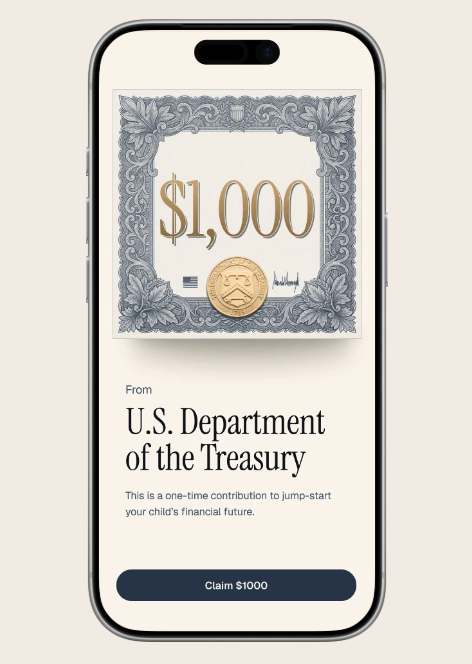
\includegraphics[width=0.9\textwidth]{fig/trump_account.png}
    \end{column}
  \end{columns}

\end{frame}

\begin{frame}{Policy: Trump Accounts}

  \begin{columns}[T]
    \begin{column}{0.55\textwidth}
      \begin{definitionbox}[Trump Accounts]
        The government deposits \textbf{\$1{,}000} into an investment account for every newborn.
        The child can access the money at \textbf{age 18}.
      \end{definitionbox}
      \begin{itemize}
        \item These accounts invest money in the stock market.
      \end{itemize}
      \vspace{0.8em}
      \begin{questionbox}
        Hypothetically, these accounts give a rate of return of 10\%. How much would \$1{,}000 grow to in 18 years?
      \end{questionbox}
    \end{column}
    \begin{column}{0.4\textwidth}
      \vspace{1em}
      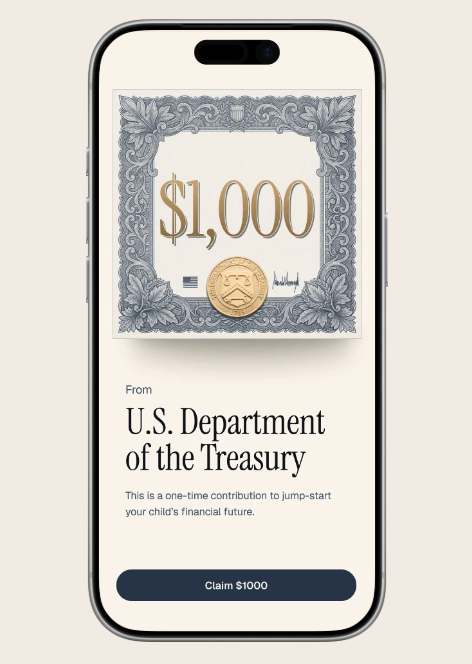
\includegraphics[width=0.9\textwidth]{fig/trump_account.png}
    \end{column}
  \end{columns}

\end{frame}

\begin{frame}{Compound Returns}

  \begin{columns}[T]
    \begin{column}{0.50\textwidth}
      \begin{methodbox}
        \centering
        {\Large $A_t = P \times (1 + r)^{t}$}

        \vspace{0.3em}
        {\small $P$ = starting amount \quad $r$ = rate of return \quad $t$ = years}
      \end{methodbox}

      \vspace{0.8em}
      \textbf{Example:} \$1{,}000 at 10\% per year.

      \vspace{0.8em}
      After 5 years:

      $A = 1{,}000 \times 1.10^{5} = \textcolor{blue}{\textbf{\$1{,}611}}$
    \end{column}
    \begin{column}{0.45\textwidth}
      \begin{tikzpicture}
        \begin{axis}[
          width=6.5cm, height=5.5cm,
          xlabel={Year}, ylabel={Balance (\$)},
          xmin=0, xmax=19, ymin=800, ymax=6000,
          xtick={0,5,10,15,18},
          grid=major, grid style={gray!20},
          xlabel style={font=\small}, ylabel style={font=\small},
          xticklabel style={font=\small}, yticklabel style={font=\small},
        ]
          \addplot[fill=blue!10, draw=none, domain=0:5, samples=30] {1000*1.10^x} \closedcycle;
          \addplot[blue, thick, domain=0:5, samples=30] {1000*1.10^x};
          \addplot[only marks, mark=*, mark size=2.5pt, blue!70!black] coordinates {(0,1000) (5,1611)};
          \node[font=\tiny, anchor=south] at (5,1611) {\$1{,}611};
        \end{axis}
      \end{tikzpicture}
    \end{column}
  \end{columns}

\end{frame}

\begin{frame}{Compound Returns}

  \begin{columns}[T]
    \begin{column}{0.50\textwidth}
      \begin{methodbox}
        \centering
        {\Large $A_t = P \times (1 + r)^{t}$}

        \vspace{0.3em}
        {\small $P$ = starting amount \quad $r$ = rate of return \quad $t$ = years}
      \end{methodbox}

      \vspace{0.8em}
      \textbf{Example:} \$1{,}000 at 10\% per year.

      \vspace{0.8em}
      After 5 years: $A = \$1{,}611$

      \vspace{0.3em}
      After 10 years:

      $A = 1{,}000 \times 1.10^{10} = \textcolor{blue}{\textbf{\$2{,}594}}$
    \end{column}
    \begin{column}{0.45\textwidth}
      \begin{tikzpicture}
        \begin{axis}[
          width=6.5cm, height=5.5cm,
          xlabel={Year}, ylabel={Balance (\$)},
          xmin=0, xmax=19, ymin=800, ymax=6000,
          xtick={0,5,10,15,18},
          grid=major, grid style={gray!20},
          xlabel style={font=\small}, ylabel style={font=\small},
          xticklabel style={font=\small}, yticklabel style={font=\small},
        ]
          \addplot[fill=blue!10, draw=none, domain=0:10, samples=30] {1000*1.10^x} \closedcycle;
          \addplot[blue, thick, domain=0:10, samples=30] {1000*1.10^x};
          \addplot[only marks, mark=*, mark size=2.5pt, blue!70!black] coordinates {(0,1000) (5,1611) (10,2594)};
          \node[font=\tiny, anchor=south] at (5,1611) {\$1{,}611};
          \node[font=\tiny, anchor=south] at (10,2594) {\$2{,}594};
        \end{axis}
      \end{tikzpicture}
    \end{column}
  \end{columns}


\end{frame}

\begin{frame}{Compound Returns}

  \begin{columns}[T]
    \begin{column}{0.50\textwidth}
      \begin{methodbox}
        \centering
        {\Large $A_t = P \times (1 + r)^{t}$}

        \vspace{0.3em}
        {\small $P$ = starting amount \quad $r$ = rate of return \quad $t$ = years}
      \end{methodbox}

      \vspace{0.8em}
      \textbf{Example:} \$1{,}000 at 10\% per year.

      \vspace{0.8em}
      After 5 years: $A = \$1{,}611$

      \vspace{0.3em}
      After 10 years: $A = \$2{,}594$

      \vspace{0.3em}
      After 18 years:

      $A = 1{,}000 \times 1.10^{18} = \textcolor{blue}{\textbf{\$5{,}560}}$

    \end{column}
    \begin{column}{0.45\textwidth}
      \begin{tikzpicture}
        \begin{axis}[
          width=6.5cm, height=5.5cm,
          xlabel={Year}, ylabel={Balance (\$)},
          xmin=0, xmax=19, ymin=800, ymax=6000,
          xtick={0,5,10,15,18},
          grid=major, grid style={gray!20},
          xlabel style={font=\small}, ylabel style={font=\small},
          xticklabel style={font=\small}, yticklabel style={font=\small},
        ]
          \addplot[fill=blue!10, draw=none, domain=0:18, samples=30] {1000*1.10^x} \closedcycle;
          \addplot[blue, thick, domain=0:18, samples=30] {1000*1.10^x};
          \addplot[only marks, mark=*, mark size=2.5pt, blue!70!black] coordinates {(0,1000) (5,1611) (10,2594) (18,5560)};
          \node[font=\tiny, anchor=south] at (5,1611) {\$1{,}611};
          \node[font=\tiny, anchor=south] at (10,2594) {\$2{,}594};
          \node[font=\tiny, anchor=south] at (18,5560) {\$5{,}560};
        \end{axis}
      \end{tikzpicture}
    \end{column}
  \end{columns}
\end{frame}

% \begin{frame}{Safe Investments: Government Bonds}

%   \begin{questionbox}
%     Where can you get a $\sim$2\% return safely?
%   \end{questionbox}
%   \pause 
%   \vspace{1em}
%   \centering
%   \begin{tikzpicture}[
%     card/.style={rounded corners=5pt, minimum width=4.2cm, minimum height=4cm,
%                  align=center, inner sep=8pt, font=\small},
%   ]
%     % Treasury Bonds
%     \node[card, draw=blue, fill=blue!8] (tbond) at (0,0) {
%       {\LARGE\textcolor{blue}{\textbf{\$}}}\\[6pt]
%       {\normalsize\textbf{Treasury Bonds}}\\[4pt]
%       {\scriptsize T-bills, T-notes}\\[2pt]
%       {\scriptsize Loans to the}\\[-1pt]
%       {\scriptsize U.S.\ government}
%     };

%     % Bank CD
%     \node[card, draw=green, fill=green!8] (cd) at (5,0) {
%       {\LARGE\textcolor{green}{\textbf{\%}}}\\[6pt]
%       {\normalsize\textbf{Bank CD}}\\[4pt]
%       {\scriptsize Certificate of Deposit}\\[2pt]
%       {\scriptsize Lock money for a}\\[-1pt]
%       {\scriptsize fixed period \& rate}
%     };

%     % Treasury ETFs
%     \node[card, draw=orange, fill=orange!8] (etf) at (10,0) {
%       {\LARGE\textcolor{orange}{\textbf{$\Sigma$}}}\\[6pt]
%       {\normalsize\textbf{Treasury ETFs}}\\[4pt]
%       {\scriptsize Pool many Treasury}\\[2pt]
%       {\scriptsize bonds together;}\\[-1pt]
%       {\scriptsize buy on stock market}
%     };
%   \end{tikzpicture}

% \end{frame}


% \begin{frame}{Answer to Q1}

%   \begin{questionbox}
%     Suppose you had \$100 in a savings account and the interest rate was 2\%
%     per year. After 5 years, how much do you think you would have?
%   \end{questionbox}
%   \pause 
%   \vspace{1em}
%   \begin{answerbox}
%     \textbf{A. More than \$102.} With compound returns, you earn returns on your
%     interest. After 5 years at 2\%:

%     \vspace{0.3em}
%     \centering $100 \times 1.02^{5} = \$110.41$

%     \vspace{0.3em}
%     \raggedright Even in just 5 years, compound interest adds more than the \$2 from the first year alone.
%   \end{answerbox}

% \end{frame}

% =============================================================================
\section{Inflation}
% =============================================================================

\begin{frame}{What Is Inflation?}

  \begin{columns}[T]
    \begin{column}{0.48\textwidth}
      \begin{definitionbox}[Inflation]
        A sustained increase in the general price level of goods and services.
        When prices rise, each dollar buys \textbf{less}.
      \end{definitionbox}

      \vspace{0.8em}
      \textbf{Example:}
      \begin{itemize}
        \item A coffee costs \$3 today.
        \item If inflation is 5\%, next year it costs \$3.15.
        \item Your dollar lost \textbf{purchasing power}.
      \end{itemize}
    \end{column}
    \begin{column}{0.48\textwidth}
      \vspace{0.5em}
      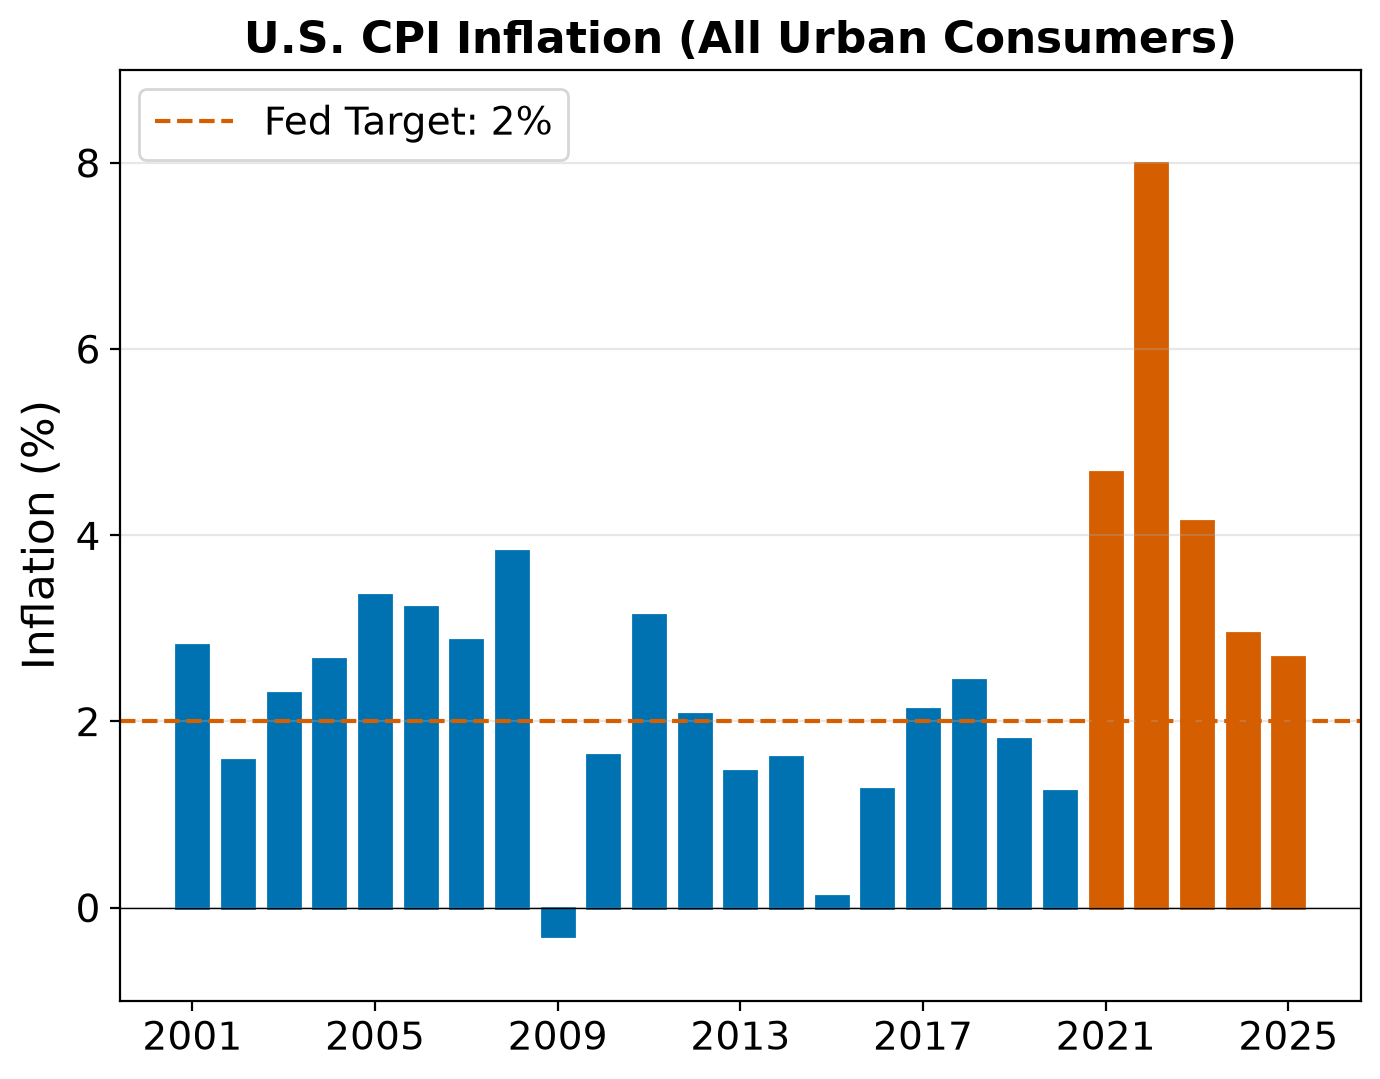
\includegraphics[width=\textwidth]{fig/cpi_inflation.png}

      \vspace{0.2em}
      {\tiny\textcolor{DarkGray}{Source: FRED, CPI-U (All Urban Consumers)}}
    \end{column}
  \end{columns}

\end{frame}

\begin{frame}{Measuring Inflation: The CPI}

  \begin{columns}[T]
    \begin{column}{0.48\textwidth}
      \begin{definitionbox}[Consumer Price Index (CPI)]
        The CPI tracks the cost of a fixed ``basket'' of goods and services
        (food, housing, gas, healthcare\ldots) that a typical household buys.
      \end{definitionbox}

      \vspace{0.8em}
      \begin{itemize}
        \item The \textbf{Bureau of Labor Statistics (BLS)} measures it monthly
        \item You can explore the data yourself at \textbf{bls.gov} and \textbf{fred.stlouisfed.org}
      \end{itemize}

      \vspace{0.8em}
      \begin{insightbox}
        If the CPI was 100 last year and is 103 this year, inflation was 3\%.
      \end{insightbox}
    \end{column}
    \begin{column}{0.48\textwidth}
      \vspace{0.5em}
      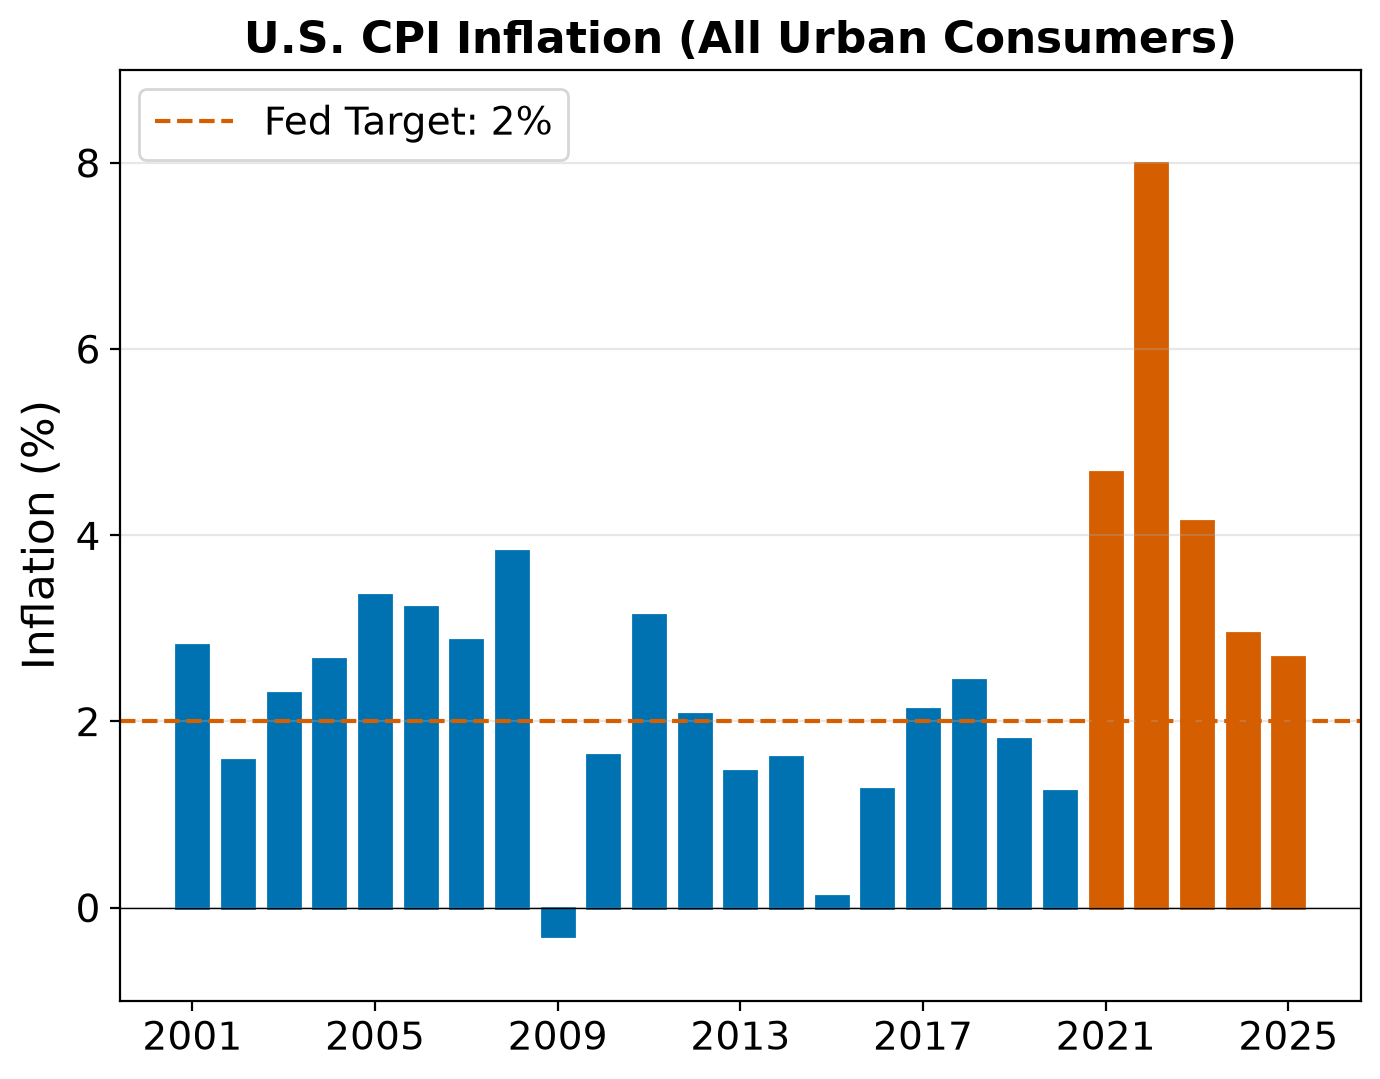
\includegraphics[width=\textwidth]{fig/cpi_inflation.png}

      \vspace{0.2em}
      {\tiny\textcolor{DarkGray}{Source: FRED, CPI-U (All Urban Consumers)}}
    \end{column}
  \end{columns}

\end{frame}


\begin{frame}{Real vs.\ Nominal Returns}

  \begin{columns}[T]
    \begin{column}{0.50\textwidth}
      \begin{methodbox}
        \centering
        {\Large Real return $\approx$ Nominal return $-$ Inflation}
      \end{methodbox}

      \vspace{0.8em}
      \textbf{Example:} Your investment returns 10\% (nominal). Inflation is 5\%.

    \end{column}
    \begin{column}{0.45\textwidth}
      \vspace{0.5em}
      % Overlay 1: Nominal line only
      \only<1>{%
      \begin{tikzpicture}
        \begin{axis}[
          width=6.5cm, height=6cm,
          xlabel={Year}, ylabel={Balance (\$)},
          xmin=0, xmax=19, ymin=800, ymax=6000,
          xtick={0,5,10,15,18},
          grid=major, grid style={gray!20},
          xlabel style={font=\small}, ylabel style={font=\small},
          xticklabel style={font=\small}, yticklabel style={font=\small},
          legend style={font=\scriptsize, at={(0.03,0.97)}, anchor=north west},
        ]
          % Nominal: 10%
          \addplot[fill=blue!10, draw=none, domain=0:18, samples=30, forget plot] {1000*1.10^x} \closedcycle;
          \addplot[blue, thick, domain=0:18, samples=30] {1000*1.10^x};
          \addlegendentry{Nominal (10\%)}
          \node[font=\tiny, blue, anchor=south] at (18,5560) {\$5{,}560};
        \end{axis}
      \end{tikzpicture}}%
      
    \end{column}
  \end{columns}

\end{frame}

\begin{frame}{Real vs.\ Nominal Returns}

  \begin{columns}[T]
    \begin{column}{0.50\textwidth}
      \begin{methodbox}
        \centering
        {\Large Real return $\approx$ Nominal return $-$ Inflation}
      \end{methodbox}

      \vspace{0.8em}
      \textbf{Example:} Your investment returns 10\% (nominal). Inflation is 5\%.

      \vspace{0.5em}

      Real return $\approx$ 10\% $-$ 5\% $=$ \textcolor{orange}{\textbf{5\%}}


      \vspace{2em}
      \begin{insightbox}
        Inflation eats into your returns. What matters is the \textbf{real return}, not the nominal one.
      \end{insightbox}
    \end{column}
    \begin{column}{0.45\textwidth}
      \vspace{0.5em}
      % Overlay 2+: Nominal + Real
      \only<1->{%
      \begin{tikzpicture}
        \begin{axis}[
          width=6.5cm, height=6cm,
          xlabel={Year}, ylabel={Balance (\$)},
          xmin=0, xmax=19, ymin=800, ymax=6000,
          xtick={0,5,10,15,18},
          grid=major, grid style={gray!20},
          xlabel style={font=\small}, ylabel style={font=\small},
          xticklabel style={font=\small}, yticklabel style={font=\small},
          legend style={font=\scriptsize, at={(0.03,0.97)}, anchor=north west},
        ]
          % Nominal: 10%
          \addplot[fill=blue!10, draw=none, domain=0:18, samples=30, forget plot] {1000*1.10^x} \closedcycle;
          \addplot[blue, thick, domain=0:18, samples=30] {1000*1.10^x};
          \addlegendentry{Nominal (10\%)}
          % Real: 5%
          \addplot[fill=orange!10, draw=none, domain=0:18, samples=30, forget plot] {1000*1.05^x} \closedcycle;
          \addplot[orange, thick, dashed, domain=0:18, samples=30] {1000*1.05^x};
          \addlegendentry{Real (5\%)}
          % Labels
          \node[font=\tiny, blue, anchor=south] at (18,5560) {\$5{,}560};
          \node[font=\tiny, orange, anchor=south] at (18,2407) {\$2{,}407};
        \end{axis}
      \end{tikzpicture}}%
    \end{column}
  \end{columns}

\end{frame}

\begin{frame}{Answer to Q1}

  \begin{questionbox}
    Suppose you had \$100 in a savings account and the interest rate was 2\%
    per year. After 5 years, how much do you think you would have?
  \end{questionbox}

  \vspace{0.5em}
  \setbeamertemplate{enumerate item}{\Alph{enumi}.}
  \begin{enumerate}
    \item More than \$102
    \item Exactly \$102
    \item Less than \$102
    \item Do not know
  \end{enumerate}

  \pause
  \vspace{0.5em}
  \begin{answerbox}
    \textbf{A. More than \$102.} With compound returns, you earn returns on your
    returns. After 5 years at 2\%:

    \vspace{0.3em}
    \centering $100 \times 1.02^{5} = \$110.41$

    \vspace{0.3em}
    \raggedright Even in just 5 years, compounding adds more than the \$2 from the first year alone.
  \end{answerbox}

\end{frame}

\begin{frame}{Answer to Q2}

  \begin{questionbox}
    Imagine that the interest rate on your savings account was 1\% per year
    and inflation was 2\% per year. After 1 year, how much would you be able
    to buy with the money in this account?
  \end{questionbox}

  \vspace{0.5em}
  \setbeamertemplate{enumerate item}{\Alph{enumi}.}
  \begin{enumerate}
    \item More than today
    \item Exactly the same
    \item Less than today
    \item Do not know
  \end{enumerate}

  \pause
  \vspace{0.5em}
  \begin{answerbox}
    \textbf{C. Less than today.} With 1\% interest and 2\% inflation, your real
    return is approximately $-1$\%.

    \vspace{0.3em}
    Your account balance grows to \$101, but the things you want to buy now
    cost \$102. You can buy \textbf{less} than before.
  \end{answerbox}

\end{frame}

% =============================================================================
\section{Bonds \& Interest Rates}
% =============================================================================

\begin{frame}{What Is a Bond?}

  \begin{columns}[T]
    \begin{column}{0.55\textwidth}
      \begin{definitionbox}[Bond]
        A bond is a \textbf{loan you make} to the government (or a company). They promise
        to pay you back with interest after a fixed period.
      \end{definitionbox}

      \vspace{0.8em}
      Think of it as an IOU:

      \vspace{0.5em}
      \begin{itemize}
        \item You give the government \$1{,}000 today
        \item In 1 year, they pay you back \$1{,}050 (that's 5\% interest)
        \item Your return: \$50
      \end{itemize}

    \end{column}
    \begin{column}{0.4\textwidth}
      \vspace{1em}
      \centering
      \begin{tikzpicture}[
        box/.style={rounded corners=4pt, minimum width=2.8cm, minimum height=1.6cm,
                    align=center, font=\small, inner sep=6pt},
      ]
        % You
        \node[box, draw=blue, fill=blue!8] (you) at (0,2.5) {
          {\normalsize\textcolor{blue}{\textbf{You}}}\\[2pt]
          {\scriptsize (investor)}
        };
        % Government
        \node[box, draw=green, fill=green!8] (gov) at (0,-1) {
          {\normalsize\textcolor{green}{\textbf{Government}}}\\[2pt]
          {\scriptsize (borrower)}
        };
        % Today arrow (money down)
        \draw[-{Stealth}, thick, blue] (-1.2,1.8) -- (-1.2,-0.3);
        \node[font=\scriptsize, blue, anchor=east, text width=1.5cm, align=center] at (-1.4,0.75) {\textbf{\$1{,}000}\\today};
        % 1 year later arrow (money up)
        \draw[-{Stealth}, thick, green] (1.2,-0.3) -- (1.2,1.8);
        \node[font=\scriptsize, green, anchor=west, text width=1.5cm, align=center] at (1.4,0.75) {\textbf{\$1{,}050}\\in 1 year};
      \end{tikzpicture}
    \end{column}
  \end{columns}
      \begin{insightbox}
        Bonds are considered safe because the government almost never fails to pay you back.
      \end{insightbox}
\end{frame}

\begin{frame}{Bond Pricing}

  \begin{columns}[T]
    \begin{column}{0.55\textwidth}
      \begin{methodbox}
        \centering
        {\Large $P = \dfrac{\text{Payout}}{1 + r}$}

        \vspace{0.3em}
        {\small $P$ = price today \quad Payout = paid in 1 year \quad $r$ = interest rate}
      \end{methodbox}

      \vspace{0.8em}
      \textbf{Example:} A bond that pays \$1{,}050 in one year.

      \vspace{0.8em}
      \begin{itemize}
        \item If $r = 5\%$: $P = \dfrac{1{,}050}{1.05} = \$1{,}000$ \pause

        \vspace{0.5em}
        \item If $r$ rises to 7\%: $P = \dfrac{1{,}050}{1.07} \approx \textcolor{vermillion}{\$981}$ \pause

        \vspace{0.5em}
        \item If $r$ drops to 3\%: $P = \dfrac{1{,}050}{1.03} \approx \textcolor{green}{\$1{,}019}$
      \end{itemize}
    \end{column}
    \begin{column}{0.4\textwidth}
      \vspace{3em}
      \begin{insightbox}
        Bond prices and interest rates move in \textbf{opposite directions}. This is one of the most important relationships in finance.
      \end{insightbox}
    \end{column}
  \end{columns}

\end{frame}

\begin{frame}{Answer to Q3}

  \begin{questionbox}
    If interest rates rise, what should happen to bond prices?
  \end{questionbox}

  \vspace{0.5em}
  \setbeamertemplate{enumerate item}{\Alph{enumi}.}
  \begin{enumerate}
    \item They should rise
    \item They should fall
    \item They should stay the same
    \item There is no relationship between bond prices and interest rates
    \item Do not know
  \end{enumerate}

  \pause
  \vspace{0.5em}
  \begin{answerbox}
    \textbf{B. They should fall.}
  \end{answerbox}

\end{frame}

% =============================================================================
\section{Stocks, ETFs \& Diversification}
% =============================================================================

\begin{frame}{What Is the Stock Market?}

  \begin{columns}[T]
    \begin{column}{0.55\textwidth}
      \begin{definitionbox}[Stock Market]
        A marketplace where people buy and sell \textbf{shares} --- small pieces
        of ownership in companies like Amazon or Google
      \end{definitionbox}

      \vspace{1em}
      When you buy a share of Amazon, you literally \textbf{own a tiny piece} of the company.

      \vspace{0.5em}
      \begin{itemize}
        \item If Amazon does well $\rightarrow$ your share becomes more valuable
        \item If Amazon does poorly $\rightarrow$ your share loses value
      \end{itemize}
    \end{column}
    \begin{column}{0.4\textwidth}
      \vspace{1em}
      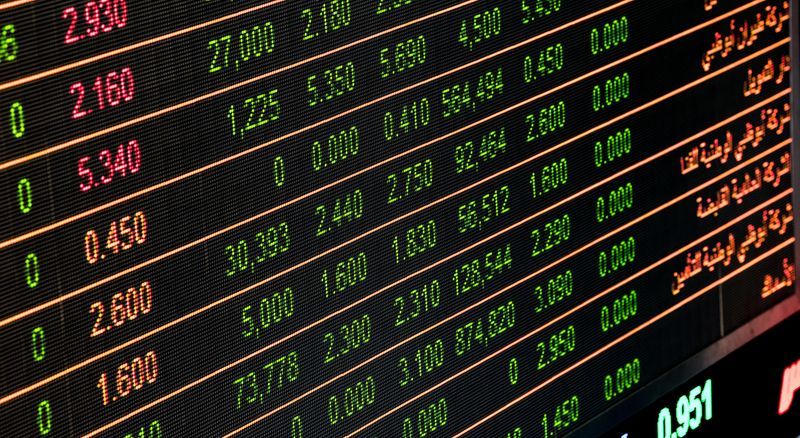
\includegraphics[width=\textwidth]{fig/stock_exchange.jpg}

      \vspace{0.3em}
      {\tiny\textcolor{lightgray}{Photo: Pexels (free license)}}
    \end{column}
  \end{columns}

\end{frame}

\begin{frame}{Single Stocks: The Upside}

  \begin{columns}[T]
    \begin{column}{0.50\textwidth}
      \vspace{0.5em}
      \textbf{Amazon} went public in 1997 for $\sim$\$0.1 per share.

      \vspace{0.8em}
      By 2025: $\sim$\$200 per share.

      \vspace{0.5em}
      That's a factor of $\times 2000$!
      \pause 
      \vspace{1em}
      \begin{insightbox}
        But could you have predicted this in 1997? For every Amazon, there are hundreds of companies that failed.
      \end{insightbox}
      \pause 
      \begin{questionbox}
        What is the stock price of a company that goes bankrupt?
      \end{questionbox}
    \end{column}
    \begin{column}{0.45\textwidth}
      \begin{tikzpicture}
        \begin{axis}[
          width=7cm,
          height=5.5cm,
          xlabel={Year},
          ylabel={Price (\$)},
          xmin=1996, xmax=2026,
          ymin=0, ymax=220,
          xtick={1997,2002,2007,2012,2017,2022},
          xticklabel style={font=\small, /pgf/number format/1000 sep={}},
          yticklabel style={font=\small},
          xlabel style={font=\small},
          ylabel style={font=\small},
          grid=major,
          grid style={gray!20},
        ]
          \addplot[green, thick, mark=*, mark size=1.5pt, smooth] coordinates {
            (1997,2) (1999,4) (2000,5) (2001,1) (2003,2.5) (2005,3)
            (2007,5) (2009,5) (2010,9) (2012,13) (2014,20)
            (2016,35) (2017,50) (2018,80) (2019,93)
            (2020,160) (2021,170) (2022,85) (2023,130) (2024,185) (2025,200)
          };
        \end{axis}
      \end{tikzpicture}

      \vspace{0.2em}
      {\tiny\textcolor{DarkGray}{Approximate split-adjusted prices}}
    \end{column}
  \end{columns}

\end{frame}

\begin{frame}{Single Stocks: The Downside}

  \begin{columns}[T]
    \begin{column}{0.5\textwidth}
      \textbf{Enron} was a Houston-based energy company that traded electricity, natural gas, and other commodities.

      \vspace{0.8em}
      \begin{itemize}
        \item 7th-largest company in America by revenue
        \item Over 20{,}000 employees
        \item Named ``America's Most Innovative Company'' by \emph{Fortune} --- six years in a row
      \end{itemize}

      \pause
      \vspace{0.8em}
      In 2001, it was revealed that executives had \textbf{hidden billions in debt} through fake partnerships. The stock went from \$90 to \textcolor{vermillion}{\textbf{zero}}.

    \end{column}
    \begin{column}{0.45\textwidth}
      \vspace{0.5em}
      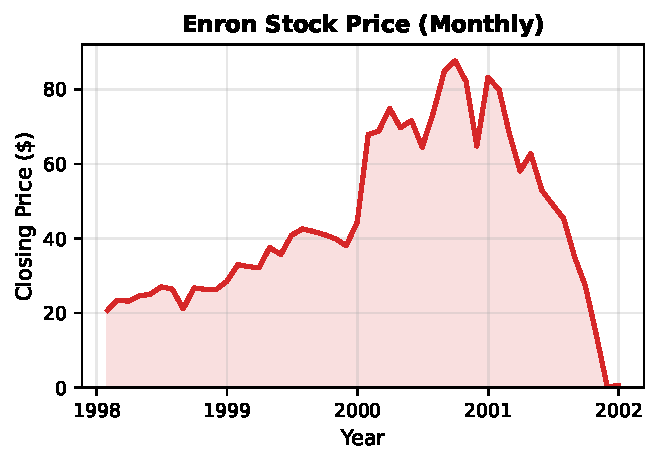
\includegraphics[width=\textwidth]{fig/enron_stock_monthly.pdf}

      \vspace{0.5em}
    \end{column}
  \end{columns}

\end{frame}

\begin{frame}{A Better Way: Funds}

  \begin{columns}[T]
    \begin{column}{0.55\textwidth}
      \begin{definitionbox}[Fund]
        A basket of many stocks bundled together. When you buy one share of a Fund,
        you own a tiny piece of \textbf{hundreds} (or thousands) of companies.
      \end{definitionbox}
      \pause
      \vspace{0.8em}
      \begin{itemize}
        \item \textbf{Example:} the S\&P 500 ETF (SPY) holds shares of the 500 largest U.S.\ companies
      \end{itemize}

      \vspace{2em}
 
    \end{column}
    \begin{column}{0.4\textwidth}
      \vspace{1em}
      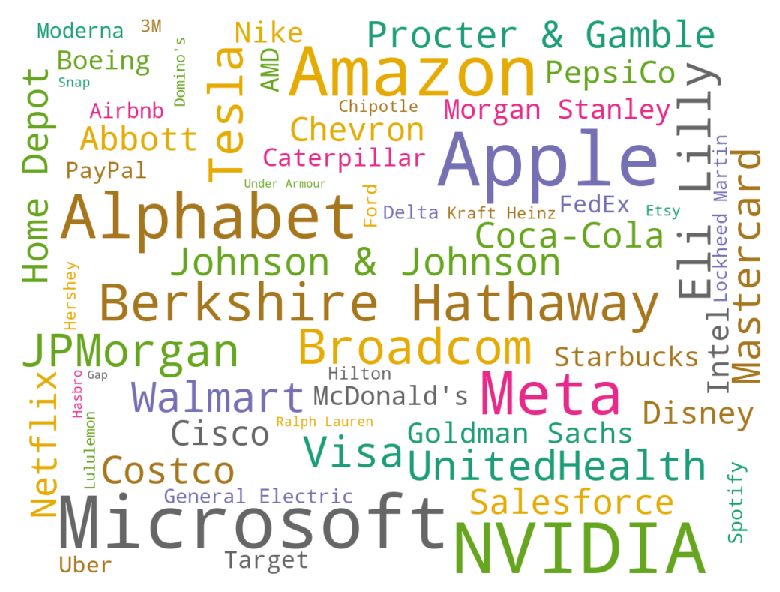
\includegraphics[width=\textwidth]{fig/sp500_wordcloud.pdf}

      \vspace{0.3em}
      \centering
      {\tiny Large public companies}
    \end{column}
  \end{columns}

\end{frame}


\begin{frame}{The Power of Diversification}

  \centering
  \begin{tikzpicture}[
    nd/.style={rounded corners=4pt, minimum width=4.5cm, minimum height=3cm,
               align=center, font=\normalsize, inner sep=8pt},
  ]
    % Single stock
    \node[nd, draw=vermillion, fill=vermillion!8] (single) at (-3.8,0) {
      \textbf{Single Stock}\\[6pt]
      {\small Company fails}\\[2pt]
      {\small $\rightarrow$ You lose \textbf{everything}}\\[6pt]
      {\large\textcolor{vermillion}{\textbf{High risk}}}
    };

    % ETF
    \node[nd, draw=green, fill=green!8] (etf) at (3.8,0) {
      \textbf{ETF (500 stocks)}\\[6pt]
      {\small One company fails}\\[2pt]
      {\small $\rightarrow$ Barely noticeable}\\[6pt]
      {\large\textcolor{green}{\textbf{Lower risk}}}
    };

    \node[font=\LARGE\bfseries, text=DarkGray] at (0,0) {vs.};
  \end{tikzpicture}

  \vspace{1.5em}
  \textbf{Diversification} means spreading your money across many investments. If one fails, the others cushion the blow.

  \begin{insightbox}
        Instead of gambling on one company, you are now betting on the whole economy. This is still a risk!
  \end{insightbox}
\end{frame}


% \begin{frame}{Trump Accounts Revisited: Savings Account vs.\ ETF}

%   \vspace{0.5em}
%   What if the Trump Account \$1{,}000 were invested in an ETF instead of a savings account?

%   \vspace{1em}
%   \begin{columns}[c]
%     \begin{column}{0.45\textwidth}
%       \begin{tcolorbox}[colback=green!8, colframe=green, title={\textbf{Savings Account (2\%)}}, fonttitle=\bfseries]
%         \centering
%         {\large $1{,}000 \times 1.02^{18}$}

%         \vspace{0.5em}
%         {\LARGE \textbf{\$1{,}428}}

%         \vspace{0.3em}
%         {\small Safe, guaranteed}
%       \end{tcolorbox}
%     \end{column}
%     \begin{column}{0.45\textwidth}
%       \begin{tcolorbox}[colback=blue!8, colframe=blue, title={\textbf{Stock ETF ($\sim$7\%)}}, fonttitle=\bfseries]
%         \centering
%         {\large $1{,}000 \times 1.07^{18}$}

%         \vspace{0.5em}
%         {\LARGE \textbf{\$3{,}380}}

%         \vspace{0.3em}
%         {\small Higher risk, higher reward}
%       \end{tcolorbox}
%     \end{column}
%   \end{columns}

%   \vspace{1em}
%   \begin{insightbox}
%     This is the fundamental trade-off in finance: \textbf{higher expected returns come with higher risk}. An ETF could more than double the payout --- but with more ups and downs along the way.
%   \end{insightbox}

% \end{frame}


\begin{frame}{Answer to Q4}

  \begin{questionbox}
    Please tell me whether this statement is true or false: ``Buying a single
    company's stock usually provides a safer return than a stock mutual fund.''
  \end{questionbox}

  \vspace{0.5em}
  \setbeamertemplate{enumerate item}{\Alph{enumi}.}
  \begin{enumerate}
    \item True
    \item False
    \item Do not know
  \end{enumerate}

  \pause
  \vspace{0.5em}
  \begin{answerbox}
    \textbf{B. False.} A single stock is \textbf{riskier} than a mutual fund.

    \vspace{0.3em}
    A mutual fund holds many stocks, so if one company fails, the impact on
    your portfolio is small. This is \textbf{diversification} --- one of the most
    important concepts in investing.
  \end{answerbox}

\end{frame}

% =============================================================================
\section{Recap}
% =============================================================================

\begin{frame}{}
  
  \centering
  \huge Let's see which team won!

\end{frame}

% NOTE: Edit the team names and scores below to match the live quiz results.
\begin{frame}{Team Results: The Quiz}

  \centering
  {\large How did each team score on the four questions?}

  \vspace{1.2em}
  \renewcommand{\arraystretch}{1.5}
  \begin{tabular}{c l c}
    \toprule
    \textbf{Place} & \textbf{Team} & \textbf{Correct (out of 4)} \\
    \midrule
    4th & Team D & 1 \\
    \pause
    3rd & Team C & 2 \\
    \pause
    2nd & Team B & 3 \\
    \pause
    $\star$ \textbf{1st} & \textbf{Team A} & \textbf{4} \\
    \bottomrule
  \end{tabular}

  \pause
  \vspace{1.2em}
  \begin{center}
    \begin{minipage}{0.7\textwidth}
      \begin{answerbox}
        \centering \textbf{Congratulations, Team A!}
      \end{answerbox}
    \end{minipage}
  \end{center}

\end{frame}

\begin{frame}{Financial Literacy in the U.S.}

  \begin{center}
    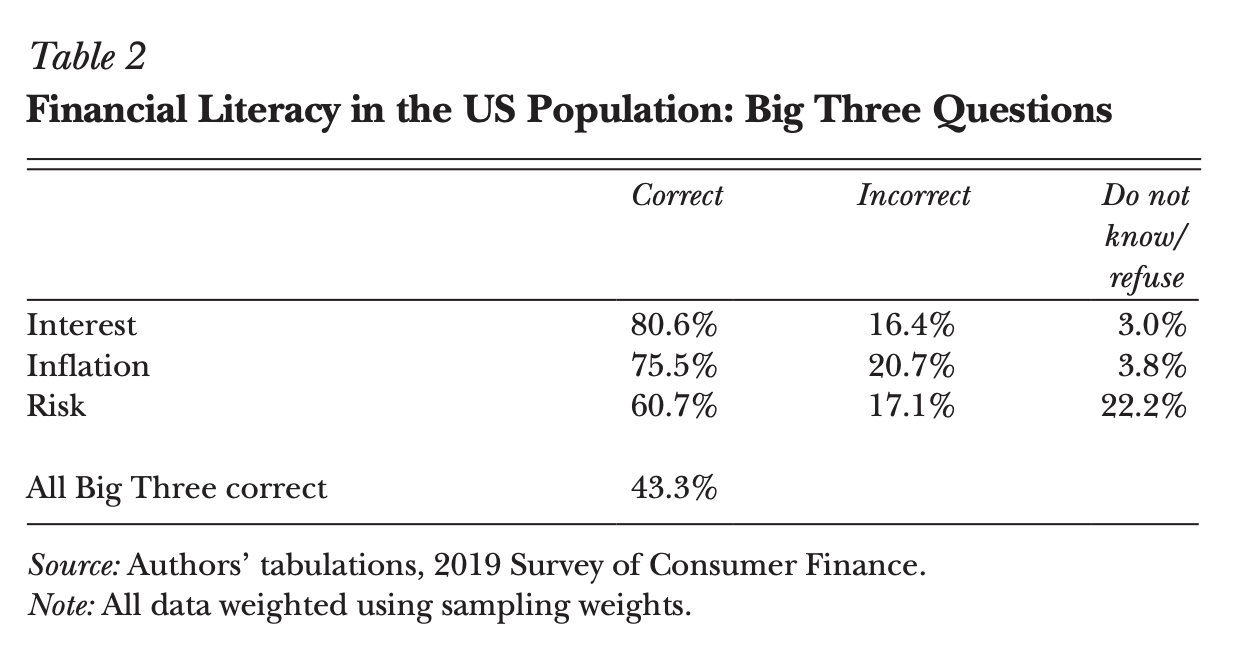
\includegraphics[width=0.85\textwidth]{fig/fin_literacy_results.png}
  \end{center}

\end{frame}

\begin{frame}{What Can You Do?}

  \begin{enumerate}
    \item \textcolor{green}{\textbf{Start saving early}} --- Compound interest rewards patience.

    \vspace{0.6em}
    \item \textcolor{orange}{\textbf{Watch inflation}} --- Make sure your returns beat it.

    \vspace{0.6em}
    \item \textcolor{blue}{\textbf{Understand bonds}} --- They're safe and good for stability.

    \vspace{0.6em}
    \item \textcolor{purple}{\textbf{Diversify with Mutual Funds or ETFs}} --- Don't bet everything on one company.

  \end{enumerate}

\end{frame}

\begin{frame}{}

  \centering
  \vspace{2em}
  {\Huge Thank you!}

  \vspace{1.5em}
  
\includegraphics[width=0.28\textwidth]{fig/qrcode_website.png}

  \vspace{0.5em}
  {\normalsize Scan to access the slides}

\end{frame}

\end{document}
